\chapter{Work Done}
\label{chapter3}

\section{During 7th Semester}
Estimating correspondences between images is one the fundamental problems in computer vision\cite{20AA} with applications ranging from large-scale 3D reconstruction to image manipulation and semantics segmentation \cite{Rubinstein2013UnsupervisedJO}.In this project, My first challenge is to build on the traditional approach and develop a convolutional neural network (CNN) architecture that mimics the standard matching process and will replace the standard local features with powerful trainable convolutional neural network features \cite{Krizhevsky2012ImageNetCW}, which allows us to handle large changes of appearance between the matched images. The outcome is a convolutional neural network architecture trainable for the end task of geometric matching,which can handle large appearance changes, and is therefore suitable for both instance-level and category-level matching problems. 

	My second task was to provide a matching layer at the end which can handle sensor interoperability issues. In heterogeneous sensor environment, it is crucial to identify the source sensor by which the acquired image is captured. This is essentially required to handle sensor interoperability issues and further in identifying various attacks on biometric systems, where biometric templates can be modified or mis-used. Another interesting application of sensor identification is in establishing the sequence of commands for law enforcement to identify spurious activities in on-line systems. An image can be altered or fabricated during the acquisition phase, transmission or during storage. In order to understand whether the image has been fabricated or not it is necessary to know the source that generates the image

	Fingerprint sensors can be classified into various categories e.g. (i) basis of imaging technology they are classified as optical, capacitive and thermal; (ii) basis of user interaction they are classified as press, sweep and non-contacted ones. Fig~\ref{fig:figure1} shows fingerprint images captured from different types of sensors. It is evident from Fig~\ref{fig:figure1}, that image quality largely depends upon underlying sensor employed.

\begin{figure}[htbp]
\centering
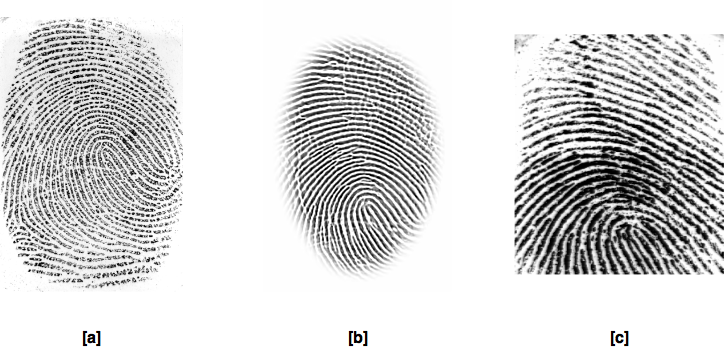
\includegraphics[scale=0.5]{./Chapter3/Figures/differentSensorsOutputs}
\caption{Example of fingerprint images taken from different sensors (a) Futronic, (b) Lumidigm, (c) SecuGen
}\label{fig:figure1}
\end{figure}


After first evaluation my work was mainly focused on providing a matching layer which can handle sensor interoperability issues. But to address this problem first we should be able to classify images on the basis of the sensors i.e. detect from which sensor the image has came. After this process the matching problem can be broken down into two (1) Inter Sensor Matching and (2) Intra Sensor Matching. The main contribution for fingerprint sensor detection is three fold, that is summarized in the following section.
	
	\begin{itemize}
		\item  An architecture based on Deep Convolutional Neural Network is proposed that is capable of detecting input fingerprint sensor by systematically pruning and training two different types of convolutional neural networks VGG and ResNet50 namely.
		\item In-depth feature analysis is done to understand the real-insight of features learned by different layers.
		\item A highly generalized deep convolutional neural network based architecture has been proposed.
	\end{itemize}

\subsection{Proposed Architecture}
In an image classification problem the task is to predict a label of the input image among the set of the predefined labels. Traditional methods of classification uses
hand-crafted features like HOG and SIFT, but these methods encode low-level characteristics and thus not able to distinguish well in case of fine grain classification problems. In present world deep learning based methods are the state of the art methods that are capable of encoding higher level characteristics
	
    Extensive experimentation has been done in order to decide the suitable network for our fine grain finger-print sensor classification problem. We have considered two networks (a) A shallow network (VGG) (b) A deep network (ResNet50) in order to understand the type of features, classification accuracy and generalization ability trade-off between shallow and deeper networks. As our finger-print sensor classification problem is not a trivial one, we are required to extract features at granular level. Another important point of consideration here is that our fingerprint image size is small and using a network having large kernel size will not be too useful. Considering all the above points in mind we conducted two set of experimentation

\subsubsection{Shallow Network (VGG-19 variant) }
	
	In the first set of experimentation we have used a variant of VGG-19 a popular deep-convolutional neural network model as shown in Fig~\ref{fig:figure2}. The foremost advantage of using this network is its small kernel filter size of 3 X 3 which tries to learn high-level features at granular levels. VGG-19 network is divided into 5-blocks with 19 weight layers. It takes an input image of size 224 X 224. After doing experimentation we have found that the block-5 is not adding any discriminative information for our fingerprint sensor classification problem so we systematically prune it and add a dropout layer also to avoid overfitting . While fine tuning this network we have used adam  optimizer with a mini-batch size of 64, initial learning rate has been set as 0.001 for 15 epoches. All the parameters that are used in this work are calculated empirically over a small validation set.

\subsubsection{Deep Network (Resnet50 variant) }
	 In the second set of experimentation our network is inspired by ResNet50 architecture. We had taken this network deliberately in order to know whether the presence of identity connections between the layers in the residual network architecture gives us an advantage in learning discriminative features for finger print sensor classification. We took pretrained ResNet50 model on ImageNet images and performed extensive experimentation over it using multi-sensor fingerprint images in order to fine tune it.
     
\subsubsection{ResNet Description and Parameterization}
The first layer of proposed architecture is an input layer which takes an input image of size 224 $\times$ 224. Given the fingerprint image and its corresponding label, the first convolutional layer CONV 1, filters the input image of size 224 $\times$ 224 using 64 kernels and pool it to an output of size 112 $\times$ 112. The filters of CONV 1 layer generally detects the edges and colors of the input image. The output of the CONV 1 is connected to max-pooling layer. After that Branch−2, Branch−3 and Branch−4 blocks of ResNet50 architecture has been utilized. At the end a fully connected layer with 2048 neuron has been added along with a dropout layer in the model with a probability of 0.4, in order to avoid over-fitting as well as to force the network to learn only robust features. Finally softmax function has been used to generate the probability distribution by minimizing the categorical cross-entropy loss-function. While fine tuning this network we have used adam optimizer with a mini-batch size of 64, initial learning rate has been set as 0.001 for 30 epochs. All the parameters that are used in this work are calculated empirically over a small validation set.

\subsubsection{ResNet Pruning}
ResNet50 is a very deep network with 50 weight layers trained over 1000 ImageNet classes. Since we have less number of classes and that too with few thousands of images, we have decide to prune the network systematically in order to avoid over-fitting. It is also famous for its notorious training hence extensive experimentation has been done to f inetune as well as systematically prune existing ResNet50 model. During experimentation we found that $Branch−2$ and $Branch−4$ of ResNet50 are extremely important for learning discriminative information, which is necessary for differentiating between images acquired from different fingerprint sensors. We also
have observed that $Branch−5$ and $Branch−3$ have “similar” contribution in final classification for our specific fingerprint sensor classification problem. Hence one can drop anyone layer, but dropping both have caused drastic performance deterioration. Hence we have dropped Branch − 5 because generated feature map size was only $7 \times 7$. \ref{fig:figure2} shows the proposed network architecture, which has been designed in a manner so that it can classify commonly used fingerprint sensors. In this model, we have dropped Branch − 5, since in our case this branch was not learning much discriminative information. By doing so, we have decreased the computation time while retaining the performance.

\begin{figure}[htbp]
\centering
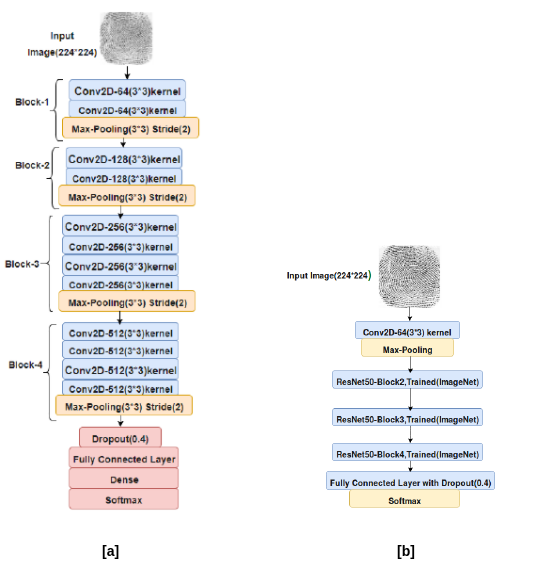
\includegraphics[scale=0.8]{./Chapter3/Figures/ModelDiagram}
\caption{ [a] VGG-19 based shallow network, [b] Resnet50 based deep network.
}\label{fig:figure2}
\end{figure}


\section{During 8th Semester}
After the start of this phase, my main aim was towards our big step Data Hashing, hence my whole work during the first month was some literature review and implementing one the papers published recently \cite{Li2018DualAD}.
The main contributions of the proposed method are shown as follows:
\begin{itemize}
	\item Two Neural Networks are trained to learn asymmetrically different hash functions. A semantic label information is used in a pairwise loss function to utilize the similarity between each pair of images.
	\item An additional asymmetric loss is applied to reveal the similarity between the binary codes and the learned features. Binary codes and real value features are bridged through an inner product, which preserves the similarity, alleviates the binary limitation, and also speeds up convergence at the training phase.
	\item To take advantage of the upper asymmetric properties, real values and discrete values are efficiently optimized through an alternate algorithm.
\end{itemize}
\subsection{Notations and Problem Definition}
Since there are two neural networks used in this paper,
X = \{$x_{1} , · · · , x_{i} , . . . , x_{N} \}  \epsilon  R^{N \times d_{1}  \times d_{2}\times 3}$ and Y = $\{y_{1} , · · · , y_{i}, . . . , y_{N} \} \epsilon R^{N\times d_{1}\times d_{2}\times 3}$  are used to denote the input images in the first and second deep neural networks, respectively, where N is the number of training samples,
$d_{1}$ and $d_{2}$ are the length and width for each image and both denote the same training data although represented by different symbols. Training samples $X$ and $Y$ are alternatively used in the first and second networks. Since our method is supervised learning, the label information can be used.
Let the uppercase letter S $\epsilon \{−1, +1\}$ denote the similarity between $X$ and $Y$ and $S_{i,j}$ is the element in the i-th row and
j-th column in S. Let $S_{i,j} = 1$ if $x_{i}$ and $y_{j}$ share the same semantic information or label, otherwise $S_{i,j} = −1$.

Denote the binary codes as $B = [b_{1} , · · · , b_{i}, . . . , b_{N} ]^T$	 $\epsilon R^{N \times k} $
 and the k-bit binary code of the i-th sample as $b_{i} \epsilon \{−1, +1\}^{k\times 1}$ . The purpose of our model is to learn two mapping functions $F$ and $G$ to project X and Y into the Hamming space B. $b_{i} = sign(F(x_{i} ))$ and $b_{j} = sign(G(y_{j} ))$,
where sign(·) is an element-wise sign function, and sign(x) =
1 if x ≥ 0, otherwise sign(x) = -1.

They have applied the convolution neural work knowing the power of deep neural network to project the information into compact codes. Feature learning is performed using the CNN-F structure. CNN-F consists of three fully connected layers as well as five convolutional layers. The network structure is listed in Table~\ref{table2}, ”st.” means the convolution stride, where ”f.” means the filter, ”LRN” means the Local Response Normalization. The last layer in the CNN-F was replaced with a k-D vector to get the final binary code and the k-bit binary codes are obtained after applying a sign operation on the output of last layer. In this proposed asymmetric structure CNN-F model is applied to both streams.


\begin{table}[th]
\centering
\caption{The Network Structure of CNN-F}
\vspace{2mm}
\label{table2}
\begin{tabular}{|l|c|}
\hline
Layer & Structure                                       \\ \hline
conv1 & f. 64 × 11 × 11; st. 4×4; pad. 0; LRN.; ×2 pool \\ \hline
conv2 & f.265 × 5 × 5; st. 1×1; pad. 2; LRN.; ×2 pool   \\ \hline
conv3 & f. 265 × 3 × 3; st. 1×1; pad. 1                 \\ \hline
conv4 & f.265 × 3 × 3; st. 1×1; pad. 1                  \\ \hline
conv5 & f. 265 × 3 × 3; st. 1×1; pad. 1; ×2 pool        \\ \hline
full6 & 4096                                            \\ \hline
full7 & 4096                                            \\ \hline
full8 & k-bit hash code                                 \\ \hline
\end{tabular}
\end{table}

\begin{figure}[htbp]
\centering
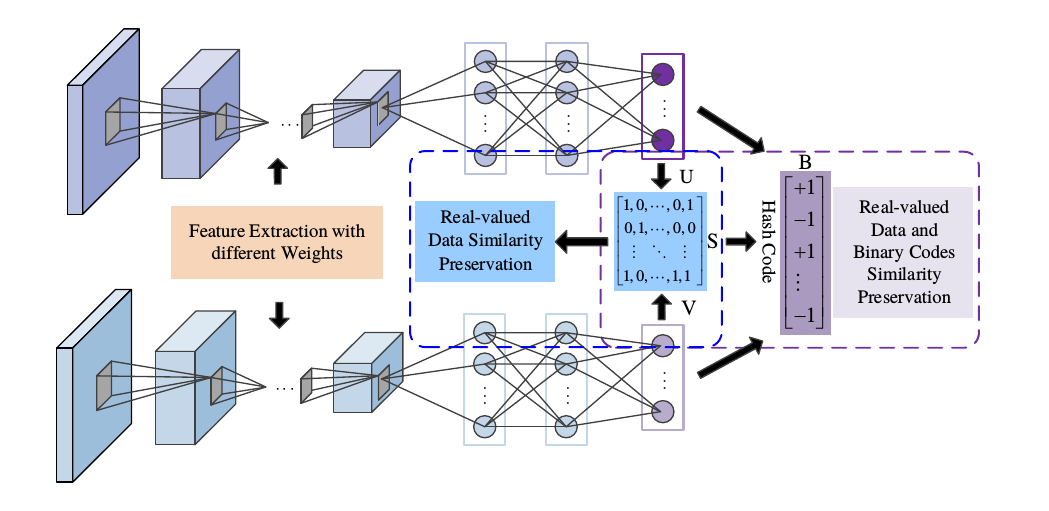
\includegraphics[scale=0.6]{./Chapter3/Figures/cnnNetwork}
\caption{ The framework of the proposed method. Two streams with five convolution layers and two full-connected layers are used for feature extraction.
}\label{fig:figure3}
\end{figure} 



\subsection{Dual Asymmetric Deep Hashing Learning}
	The main framework of the proposed method is shown in Fig~\ref{fig:figure3}. As we can see, there are two end-to-end neural networks to discriminatively represent the inputs. For a pair of outputs F and G in these two streams, their semantic information is exploit through a pairwise loss according to their predefined similarity matrix. Since the purpose is to
obtain hash functions through the deep networks, the binary code B is also generated by minimizing its distance between
F and G. Furthermore, in order to preserve the similarity between the learned binary codes and real-value features, and
alleviate the binary limitation, another asymmetric pairwise loss is introduced by using the inner product of the hash codes
B and learned features $F (G)$

Denote $f (x_{i}, W_{f} )$ $\epsilon R^{k\times 1}$ as the output of the i-th sample in the last layer of the first stream, where $W_{f}$ is the parameter of the network. To simplify the notation, we use $f_{i}$ to replace $f (x_{i}, W_{f} )$. Similarly, we can obtain the output $g_{j}$ corresponding to the j-th sample under the parameter $W_{g}$ in the second network. Thus, the features $F = [f_{1} , · · · , f_{i} , f_{n} ]^T \epsilon R^{n\times k}$ and $G = [g_{1}, · · · , g_{i} , g_{n}]^T \epsilon R^{n\times k}$ corresponding to the first and second networks are then gained.
To learn an accurate binary code, we set $sign(f_{i})$ and $sign(g_{i})$ to be close to their corresponding hash code $b_{i}$ . A
general way is to minimize the L2 loss between them.

\begin{equation}
	    min \vert \vert sign(f_{i}) - b_{i} \vert \vert ^2 _{2} + \vert \vert sign(g_{i}) - b_{i} \vert \vert^2_{2}
\label{eq1}
\end{equation}
However, it is difficult to make a back-propagation for the gradient with respect to $f_{i}$ or $g_{i}$ since their gradients are zero anywhere. In this paper, we apply $tanh(·)$ to softly approximate the $sign(·)$ function. Thus, equation is transformed into

\begin{equation}
	    min \vert \vert tanh(f_{i}) - b_{i} \vert \vert ^2 _{2} + \vert \vert tanh(g_{i}) - b_{i} \vert \vert^2_{2}
\label{eq2}
\end{equation}

Although previous equation achieves to approximate discrete codes but the similarity between the binary codes and real-value features is ignored. To tackle this problem, another asymmetric pairwise loss is introduced.

\begin{equation}
	    min \vert \vert tanh({f_{i}}^T)b_{j} - kS_{ij} \vert \vert ^2 _{2} + \vert \vert tanh({g_{i}}^T)b_{j} - kS_{ij} \vert \vert^2_{2}
\label{eq3}
\end{equation}

In above Eq., the similarity between the real-valued data and binary codes is measured by their inner product. It is easy to observe that above Eq. not only encourages the $tanh(f_{i} ) (tanh(g_{i} ))$ and $b_{i}$ to be consistent, but also preserve the similarity between them.
Jointly taking all the equations into account, the objective function can be obtained as follows:


\begin{equation}
	\begin{aligned}
	    min_{F,G,B}  L = \vert \vert tanh(F)B^T - kS \vert \vert ^2 _{F} + \vert \vert tanh(G)B^T - kS \vert \vert^2_{F} 
	    \\- \tau \sum\limits_{i,j=1}^n (S_{ij}\theta_{ij} - log(1 + \exp^{\theta_{ij}})) 
	    \\+ \gamma (\vert \vert tanh(F) - B \vert \vert^2_{F} + \vert \vert tanh(G) - B\vert \vert^2_{F}) 
	    \\+ \eta(\vert \vert tanh(F)^T1\vert\vert^2_{F} + \vert\vert tanh(G)^T1 \vert \vert^2_{F})
	   \end{aligned}
\label{eq4}
\end{equation}


where $\tau$ , $\gamma$ and $\eta$ are the non-negative parameters to make a trade-off among various terms. Note that the purpose of the
forth term $\vert \vert tanh(F)^T1 \vert \vert^2_{F} + \vert \vert tanh(G)^T1 \vert \vert^2_{F}$ in the objective. function is to maximize the information provided by each bit. In detail, this term makes a balance for each bit, which encourages the number of -1 and +1 to be approximately similar among all training samples.
